\documentclass[11pt,titlepage]{article}
\usepackage{amsmath,amssymb,amstext,mathtools,amsthm}
\usepackage{xcolor}
\usepackage[utf8]{inputenc}
\usepackage[ngerman]{babel}
\usepackage[paper=a4paper,left=25mm,right=25mm,top=25mm,bottom=25mm]{geometry}
\usepackage{geometry}
\usepackage{hyperref}
\hypersetup{bookmarksnumbered}

\usepackage{dsfont}
%\usepackage{xfrac}
\usepackage{tikz}
\usepackage{graphicx}
\usepackage{bigints}
\usepackage{bibgerm}

\usetikzlibrary{positioning}
%\usetikzlibrary{arrows}

\newcommand{\setN}{\mathbb{N}}
\newcommand{\setZ}{\mathbb{Z}}
\newcommand{\setQ}{\mathbb{Q}}
\newcommand{\setR}{\mathbb{R}}
\newcommand{\setC}{\mathbb{C}}
\newcommand{\setH}{\mathbb{H}}
\newcommand{\setI}{\mathbb{I}}
\newcommand{\abs}[1]{{\left| #1 \right|}}

\theoremstyle{definition}
\newtheorem{theorem}{Satz}[section]
\newtheorem{corollary}[theorem]{Folgerung}
\newtheorem{proposition}[theorem]{Proposition}
\newtheorem{lemma}[theorem]{Lemma}
\newtheorem{definition}[theorem]{Definition}
\newtheorem{example}[theorem]{Beispiel}
\newtheorem*{axiom}{Axiom}
\newtheorem{remark}[theorem]{Bemerkung}

\theoremstyle{remark}
\newtheorem*{repetition}{Wiederholung}
\newtheorem*{remind}{Erinnerung}

\title{Dehn-Invariante}
\author{Jannis Klingler}
\date{\today}

\begin{document}

	\maketitle
	
	\tableofcontents
	
	\newpage
	
	\section{Zerlegungsgleichheit und Ergänzungsgleichheit von Polytopen}
	
	\subsection{Polytope}
	
	\begin{repetition}[Dual-Raum]
		Der Dualraum $V^*$ eines $k$-Vektorraums $V$ ist die Menge aller linearen Abbildungen von $V$ in den Körper 	$k$.
	\end{repetition}
	
	\begin{definition}[Halbraum]
		Ein Halbraum in einem reellen Vektorraum ist eine Teilmenge der Form
		\[ H= \{ v\in V \  \vert\  \alpha(v)\leq r \}, \]
		wobei $\alpha\in V^*\setminus\{0\}$ und $r\in\setR$.
	\end{definition}
	
	\begin{definition}[konvexes Polytop]
		Ein konvexes $d$-Polytop $P$ in einem $d$-dimensionalen reellen Vektorraum $V$ ist der Schnitt endlich vieler 
		Halbräume. $P$ ist beschränkt, falls für jedes $\alpha\in V^*\setminus\{0\}$ ein $r\in \setR$ existiert, sd. 
		$\alpha(x)\leq r$ für alle $x\in P$ gilt.
	\end{definition}
	
	\begin{definition}[Polytop]
		Ein $d$-Polytop $P$ in einem $d$-dimensionalen reellen Vektorraum ist die Vereinigung endlich vieler 
		konvexer $d$-Polytope. \\
		Für $d=0$ ist $P$ eine Ecke, für $d=1$ ist $P$ eine Strecke, für $d=2$ ist $P$ ein Polytop und für $d=3$ 
		ist $P$ ein Polyeder.
	\end{definition}
	
	\begin{definition}[Kongruenz]
		Wir nennen zwei Polytope $P$ und $Q$ \textsl{kongruent}, wenn es eine Isometrie $g$ gibt, sd. 
		$g(P)=Q$. Eine Isometrie ist hierbei eine Abbildung, die die Abstände zweier beliebiger Punkte erhält. 
		Wir schreiben dann $P\cong Q$.
	\end{definition}
	
	Im folgenden meinen wir mit $P_1+\ldots+P_n$ die disjunkte Vereinigung.
	
	\begin{definition}[Zerlegungsgleichheit]
		Zwei $d$-Polytope $P$ und $Q$ heißen \textsl{zerlegungsgleich}, wenn es endlich viele $d$-Polytope 
		$P_1,\ldots,P_n,Q_1,\ldots,Q_n$ mit $P=P_1 +\ldots +P_n$,  $Q=Q_1 +\ldots+Q_n$ 
		gibt, sd. 
		\[P_i\cong Q_i\]
		für alle $i\in\{1,\ldots,n\}$. Wir schreiben $P\sim Q$.
	\end{definition}
	
	\begin{definition}[Ergänzungsgleich]
		Zwei $d$-Polytope $P$ und $Q$ heißen \textsl{ergänzungsgleich}, wenn es endlich viele $d$-Polytope 
		$P_1,\ldots,P_n$, $Q_1,\ldots,Q_n$ gibt, wobei gilt $P_i\cong Q_i$ für alle $i\in\{1,\ldots,n\}$, sd. die Polytope
		\[P'=P+P_1+\ldots+P_n,\qquad Q'=Q+Q_1+\ldots+Q_n\]
		zerlegungsgleich sind.
	\end{definition}
	
	Man sieht leicht, dass folgendes gilt:
	
	\begin{proposition} \label{prop:zerl,erg}
		Zerlegungsgleiche Polytope sind ergänzungsgleich.
	\end{proposition}
	
	\begin{proof}
		Klar.
	\end{proof}
	
	\subsection{Bolyai-Gerwien Theorem}
	
	\begin{lemma} \label{lemma:transitiv}
		Seien $P$, $Q$ und $R$ Polygone und es gilt $P\sim Q$ und $Q\sim R$. Dann folgt $P\sim R$.
	\end{lemma}
	
	\begin{proof}
		Seien die Zerlegungen der Polygone wie folgt gegeben
		\begin{align*}
			P &= P_1+\ldots+P_n \\
			Q &= Q_1+\ldots+Q_n = Q_1'+\ldots+Q_m' \\
			R &= R_1+\ldots+R_m,
		\end{align*}
		wobei $P_i\cong Q_i$ für alle $i\in\{1,\ldots,n\}$ und $Q_j'\cong R_j$ für alle $j\in\{1,\ldots,m\}$. 
		Seien $f_1,\ldots,f_n$ die Isometrien, die alle $P_i$ in $Q_i$ überführen (d. h. $f_i(P_i)=Q_i$) und 
		$g_1,\ldots,g_m$ die Isometrien, die alle $Q_j'$ in $R_j$ überführen (d. h. $g_j(Q_j')=R_j$).
		Wir definieren
		\[ F_{ij}:=Q_i\cap Q_j',\]
		für $i\in\{1,\ldots,n\}$ und $j\in\{1,\ldots,m\}$ (Beachte, dass $F_{ij}$ leer sein kann). Zwei verschiedene 
		$F_{ij}$ sind disjunkt, denn für $i_1,i_2\in\{1,\ldots\,n\}$ mit $i_1\neq i_2$ gilt $F_{i_1 j}\subset Q_{i_1}$, 
		$F_{i_2 j}\subset Q_{i_2}$ und da $Q_{i_1}$ und $Q_{i_2}$ disjunkt sind folgt, dass $F_{i_1 j}$ und 
		$F_{i_2 j}$ disjunkt sind. Außerdem gilt
		\[\bigcup_{j=1}^m F_{ij} = \bigcup_{j=1}^m \left( Q_i \cap Q_j' \right) = Q_i \cap \left( \bigcup_{j=1}^m Q_j' \right)
		=Q_i \cap Q = Q_i. \]
		Also lassen sich $P$ und $R$ folgendermaßen darstellen
		\[ P=\bigcup_{i=1}^n P_i = \bigcup_{i=1}^n f_i(Q_i) =\bigcup_{i=1}^n f_i \left(\bigcup_{j=1}^m F_{ij} \right) =
		\bigcup_{i=1}^n \bigcup_{j=1}^m f_i(F_{ij}), \]
		und
		\[ R=\bigcup_{i=1}^n \bigcup_{j=1}^m g_j(F_{ij}). \]
		Als letztes überlegen wir uns, dass gilt $f_i(F_{ij})\cong g_j(F_{ij})$. Betrachte hierzu die Isometrie 
		$g_j\circ f_i^{-1}$, dann gilt $g_j(f_i^{-1}(f_i(F_{ij})))=g_j(F_{ij})$. Also finden wir für $P$ und $R$ jeweils eine 
		Zerlegung aus kongruenten Polygonen und damit sind auch $P$ und $R$ zerlegungsgleich bzw. $P\sim R$.
	\end{proof}
	
	\begin{lemma}
		Sei $P$ ein beliebiges Polygon, dann lässt sich $P$ in eine endliche Anzahl von Dreiecken zerlegen.
	\end{lemma}
	
	\begin{proof}
		Kommt noch.
	\end{proof}
	
	\begin{lemma}
		Sei $P$ ein Dreieck, dann gibt es ein Rechteck $Q$, sd. $P\sim Q$. \label{lemma:dreieck,rechteck}
	\end{lemma}
	
	\begin{proof}
		Sei $P$ das Dreieck mit den Ecken $a,b,c$ und sei o.B.d.A $\overline{ab}$ die längste Seite. Wir zeichnen 
		nun die Lotstrecke auf der Strecke $\overline{ab}$ durch den Punkt $c$ ein und nennen den Lotfußpunkt $d$. 
		Der Punkt $d$ liegt auf der Strecke $\overline{ab}$, da sonst $\overline{ab}$ nicht die längste Seite war. 
		Nun halbieren wir die Lotstrecke $\overline{cd}$ und zeichnen die Lotgerade $\overline{mn}$ auf der 
		Strecke $\overline{cd}$ durch den Mittelpunkt $e$ der Strecke ($m$ und $n$ sind hierbei die Schnittpunkte 
		dieser Lotgeraden mit dem Dreieck $P$). Da $\overline{cd}$ senkrecht auf $\overline{ab}$ und $\overline{mn}$ 
		senkrecht auf $\overline{cd}$ ist, sind $\overline{ab}$ und $\overline{mn}$ parallel. Wir bilden erneut die 
		Lotgeraden auf $\overline{ab}$ durch die Punkte $a$ und $b$ und nennen den Schnittpunkt der Lotgerade 
		durch $a$ mit der Gerade, die durch $m$ und $n$ verläuft, $f$ und den Schnittpunkt der Lotgerade durch 
		$b$ mit der Gerade, die durch $m$ und $n$ verläuft, $g$. Dadurch erhalten wir ein Rechteck $Q$ mit den 
		Eckpunkten $a,b,f,g$. Wir stellen fest, dass die Dreiecke mit den Eckpunkten $m,e,c$ und $a,m,f$, welche in 
		Abbildung \ref{Abb.1} grau hinterlegt sind, kongruent sind. Weiterhin sind die Dreiecke mit den Eckpunkten 
		$e,n,c$ und $b,g,n$, welche weiß hinterlegt sind, kongruent. Damit lassen sich $P$ und $Q$ in die beiden 
		kongruenten Dreiecke und den schraffierten Trapezoid, mit den Eckpunkten $a,b,n,m$, zerlegen und sind somit 
		zerlegungsgleich.
	\end{proof}
	
	\begin{figure}[!htbp]
		\centering
		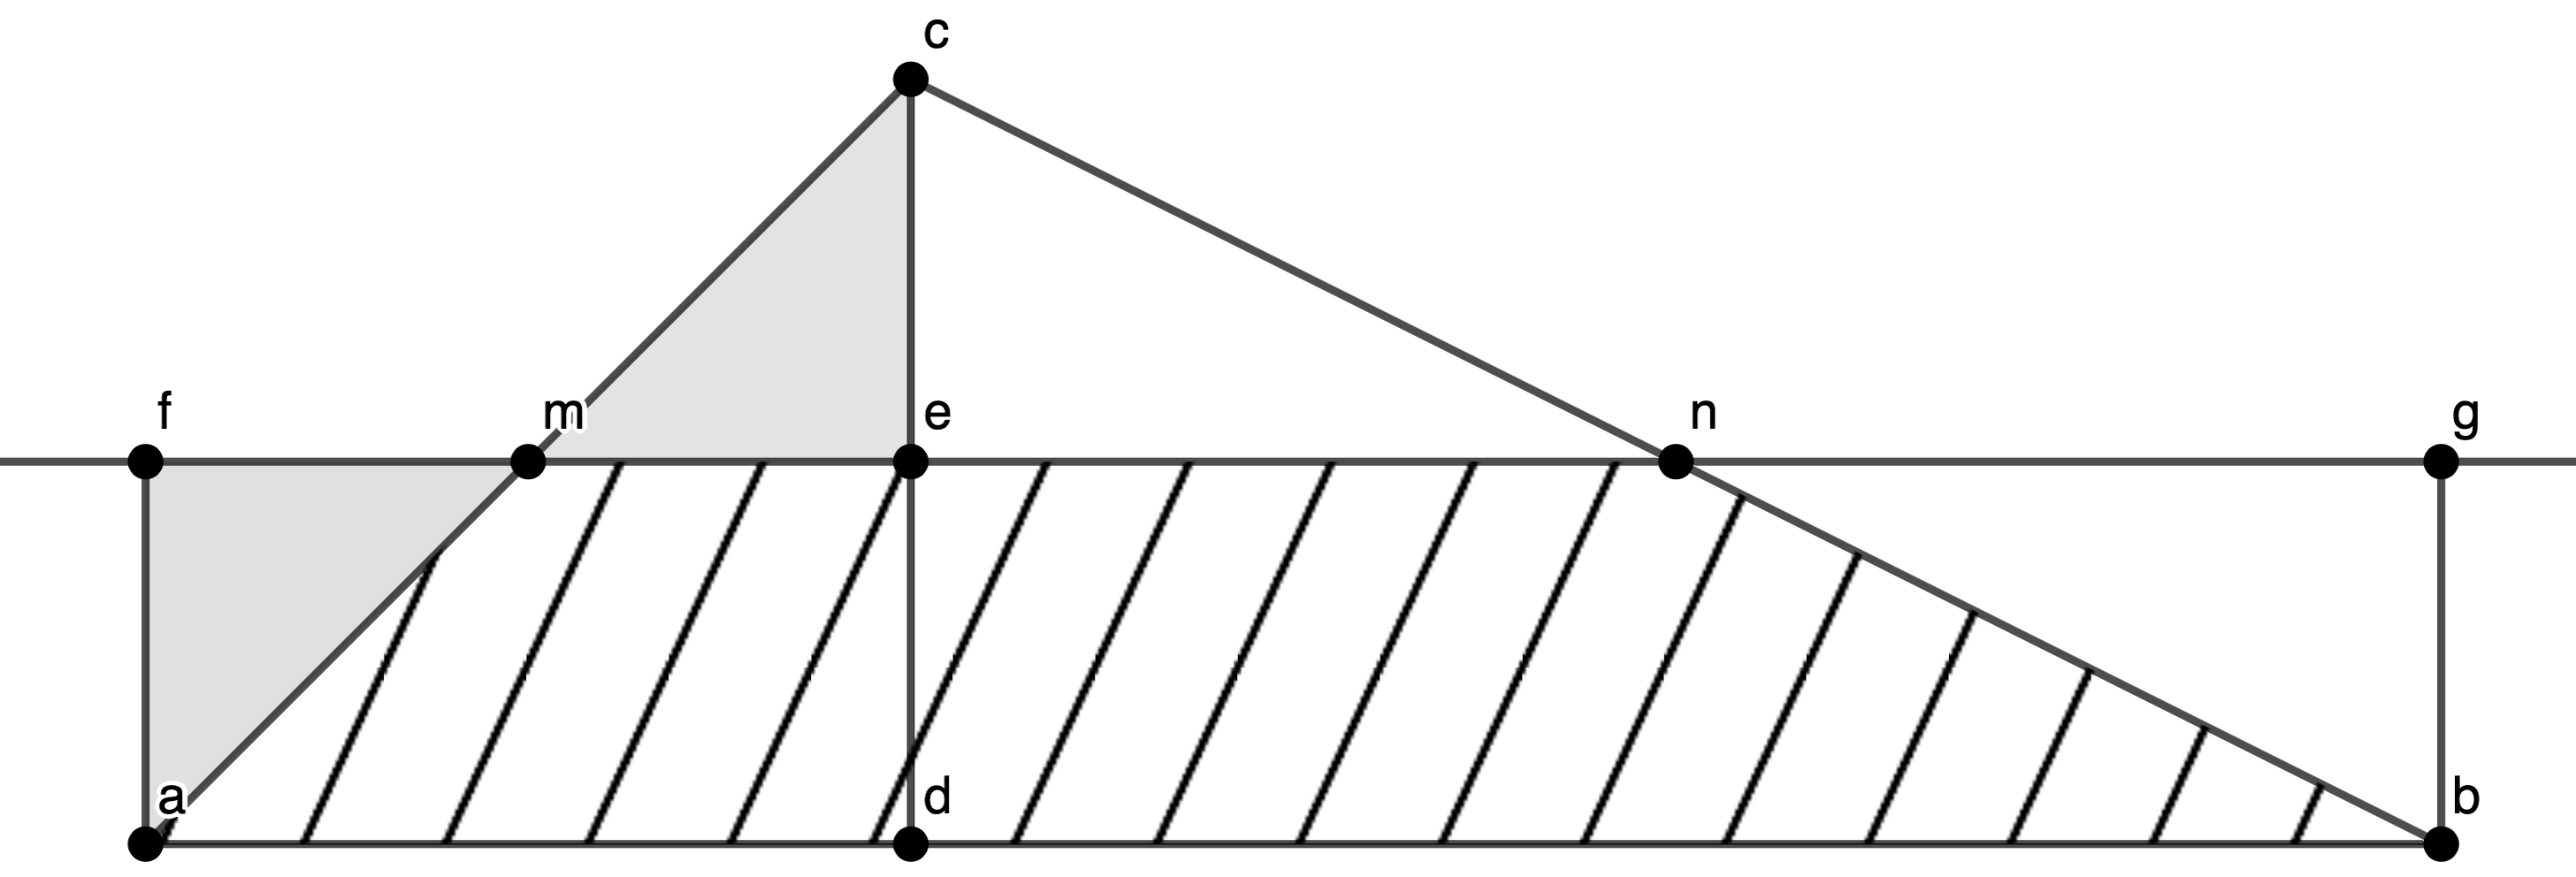
\includegraphics[scale=1.6]{DreieckLemma}
		\caption{Zerlegung eines Dreiecks in ein Rechteck}
		\label{Abb.1}
	\end{figure}
	
	\begin{lemma} \label{lemma:rechtecke}
		Zwei beliebige Rechtecke mit dem gleichen Flächeninhalt, sind zerlegungsgleich.
	\end{lemma}
	
	\begin{proof}
		Seien $P$ und $Q$ zwei Rechtecke mit dem gleichen Flächeninhalt, d. h. falls $h_P$ die Höhe und 
		$b_P$ die Breite des Rechtecks $P$ und $h_Q$ die Höhe und $b_Q$ die Breite des Rechtecks $Q$ sind, 
		dann soll gelten $h_P \cdot b_P = h_Q \cdot b_Q$ also auch
		\begin{align}
			\frac{b_P}{h_Q}=\frac{b_Q}{h_P}. \label{lemma:rechteck;1}
		\end{align}
		\begin{figure}[!htbp]
			\centering
			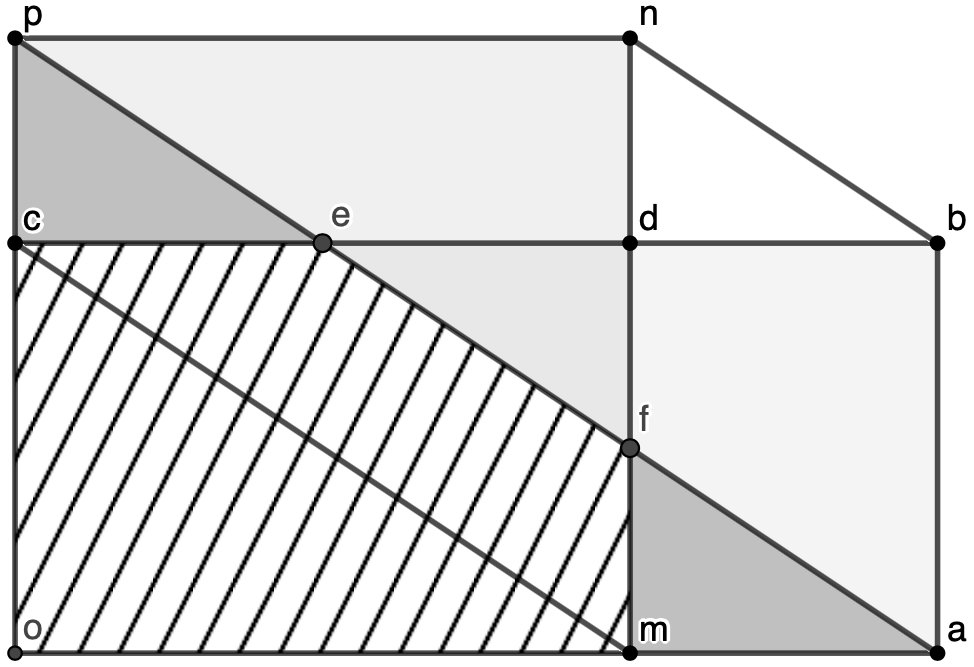
\includegraphics[scale=1.4]{Rechteck}
			\caption{Zerlegung zweier Rechtecke}
			\label{Abb.2}
		\end{figure}
		Seien $o,a,b,c$ die Eckpunkte des Dreiecks $P$ und $o,m,n,p$ die Eckpunkte des Dreiecks $Q$, siehe 
		Abbildung \ref{Abb.2}. 
		Wir verschieben hier $Q$ so auf auf $P$, dass beide eine gemeinsame Ecke $o$ mit rechtem Winkel haben. 
		Dies ändert nichts am Resultat. 
		Die Höhe $h_P$ soll also der Länge der Strecken $\overline{co}$ und $\overline{ab}$ entsprechen. Die 
		Breite $b_P$ soll der Länge der Strecken $\overline{oa}$ und $\overline{bc}$ entsprechen. Analog soll 
		$h_Q$ der Länge der Strecken $\overline{po}$ und $\overline{mn}$ und $b_Q$ der Länge der Strecken 
		$\overline{om}$ und $\overline{np}$ entsprechen. Wegen \ref{lemma:rechteck;1} sehen wir also, dass 
		die Strecken $\overline{mc}$ und $\overline{ap}$ parallel sind. Außerdem stellen wir fest, dass gilt
		\[ (b_P-b_Q)h_P=b_P h_P-b_Q h_P=h_Qb_Q-b_Qh_P=b_Q(h_Q-h_P) \]
		also auch
		\[\frac{b_P-b_Q}{h_Q-h_P}=\frac{b_Q}{h_P}. \]
		Damit folgt, dass die Dreiecke $oap$ und $dbn$ ähnlich sind und folglich sind die Strecken $\overline{ap}$ 
		und $\overline{nb}$ parallel. Hierbei sei $d$ der Schnittpunkt der Strecken $\overline{mn}$ und 
		$\overline{bc}$. Also sind die drei Strecken $\overline{mc}$, $\overline{ap}$ und $\overline{nb}$ 
		parallel. Nun unterscheiden wir zwei Fälle
		\begin{enumerate}
			\item \textsl{Fall:} Die Verbindungsstrecke $\overline{ap}$ der Eckpunkte schneidet das 
			Rechteck $omdc$ in den Punkten $e$, mit der Seite $\overline{dc}$ und $f$, mit der Seite $\overline{md}$ 
			, siehe Abbildung \ref{Abb.2}. Es gilt $2b_Q\geq b_P$.
			Also sind die beiden in der Abbildung grau hinterlegten Dreiecke $maf$ und $cep$ und die beiden 
			in der Abbildung hellgrau hinterlegten Dreiecke $abe$ und $fnp$ kongruent. Mit dem übrig gebliebenen 
			in der Abbildung schraffierten Fünfeck $omfec$ ist unsere Zerlegung komplett.
			
			\item \textsl{Fall:} Die Verbindungsstrecke $\overline{ap}$ der Eckpunkte schneidet das 
			Rechteck $omdc$ nicht, siehe Abbildung \ref{Abb.3}. 
			Es gilt also $2b_Q<b_P$. Sei nun $e$ hierbei der Mittelpunkt der Strecke $\overline{oa}$ und $k$ die 
			kleinste natürliche Zahl, wie oft man die Strecke $\overline{om}$ entlang der Strecke $\overline{oa}$ 
			legen muss, sd. wir einen Punkt $t$ erhalten der nicht mehr auf der Strecke $\overline{oe}$ liegt 
			sondern auf der Strecke $\overline{ea}$. Nun zerlegen wir das Rechteck $Q$ in $k$ Rechtecke, deren 
			Basis parallel ist zur Strecke $\overline{om}$, die wir nun entlang der neu enstandenen Strecke 
			$\overline{ot}$ legen. Wir erhalten, somit das zu $Q$ zerlegungsgleiche Rechteck $otuv$. 
			Sei die Breite dieses Rechtecks nun $b'$, die offensichtlich die Bedingung
			\[ 2b'>b_P \]
			erfüllt. Damit können wir nach dem ersten Fall sagen, dass die Rechtecke $P$ und $otuv$ 
			zerlegungsgleich sind. Nach Lemma \ref{lemma:transitiv} sind also auch $P$ und $Q$ zerlegungsgleich.
		\end{enumerate}
		Damit sind $P$ und $Q$ zerlegungsgleich.
	\end{proof}
	
	\begin{figure}[!htbp]
		\centering
		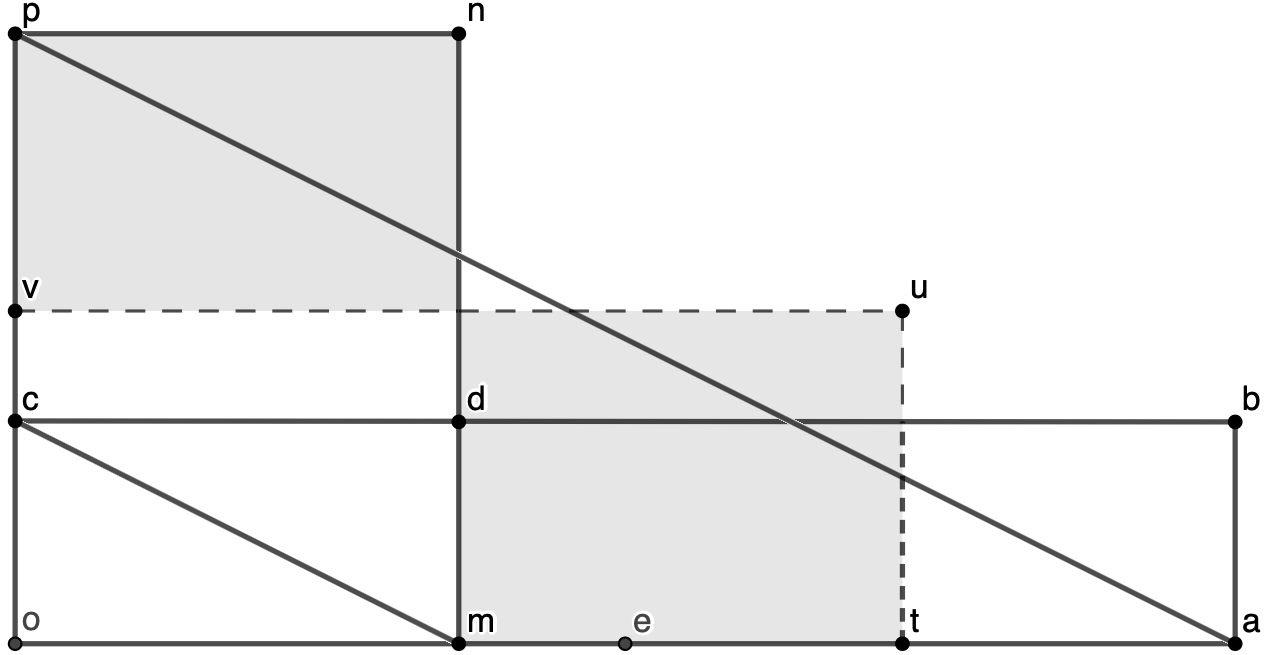
\includegraphics[scale=0.8]{Rechteck2}
		\caption{Zerlegung zweier Rechtecke}
		\label{Abb.3}
	\end{figure}
	
	\begin{theorem}[Bolyai-Gerwien Theorem] \label{theorem:bolyai-gerwien}
		Zwei beliebige Polygone mit dem gleichen Flächeninhalt sind zerlegungsgleich.
	\end{theorem}
	
	\begin{proof}
		Sei $P$ ein Polygon. Dann kann $P$ in endlich viele disjunkte Dreiecke zerlegt werden und jedes dieser 
		Dreiecke ist nach Lemma \ref{lemma:dreieck,rechteck} zerlegungsgleich zu einem Rechteck. Wir finden 
		also für $P$ die Darstellung
		\[ P\sim P_1+\ldots+P_n,\]
		wobei $P_1,\ldots,P_n$ Rechtecke sind. Nun nehmen wir eine beliebige Kante $\overline{a_0b_0}$ und 
		stellen die Lotgeraden auf den Eckpunkten $a_0$ und $b_0$ auf. Anschließend ziehen wir $n$ 
		parallele Strecken zu $\overline{a_0b_0}$, sd. der Flächeninhalt des Recheckts $a_{i-1}b_{i-1}b_ia_i$, 
		welches wir $R_i$ nennen, dem Flächeninhalt des Rechtecks $P_i$ entspricht, wobei $i=1,\ldots,n$. 
		Nach Lemma \ref{lemma:rechtecke} gilt also $P_i\sim R_i$ für alle $i$ und damit
		\[ P_1+\ldots+P_n\sim R_1+\ldots+R_n. \]
		Da $P\sim P_1+\ldots+P_n$ gilt also mit Lemma \ref{lemma:transitiv}
		\[ P\sim R_1+\ldots+R_n\]
		und damit zum Rechteck $a_0b_0b_na_n$. Damit ist jedes Polygon zerlegungsgleich mit einem Rechteck. \\
		Seien nun $P$ und $Q$ zwei Polygone mit gleichem Flächeninhalt, dann finden wir wie oben gezeigt 
		Rechtecke $R_1$ und $R_2$, sd.
		\[ P\sim R_1,\quad Q\sim R_2.\]
		Nach Lemma \ref{lemma:rechtecke} gilt also nun auch $R_1\sim R_2$ und damit folgt mit Lemma 
		\ref{lemma:transitiv} $P\sim Q$.
	\end{proof}
	
	Wir haben also nun gesehen, dass sich jedes beliebige Polygon in Dreiecke zerlegen lässt. Diese Dreiecke 
	sind nach Lemma \ref{lemma:dreieck,rechteck} zerlegungsgleich Rechtecken mit gleichem 
	Flächeninhalt. Zuletzt können wir mit Satz \ref{theorem:bolyai-gerwien} die Rechtecke in normierte Rechtecke (d. h. 
	Rechtecke mit Höhe $1$)
	zerlegen. Haben wir nun zwei beliebige Polygone $P$ und $Q$ mit gleichem Flächeninhalt $a$ gegeben, so sind 
	beide Polygone 
	nach Lemma \ref{lemma:transitiv} zerlegungsgleich mit einem normierten Rechteck $R$, das die Breite $a$ hat und 
	wiederum folgt mit der Transitivität der Zerlegungsgleichheit, dass $P$ und $Q$ zerlegungsgleich sind. Damit sind 
	zwei beliebige Polygone zerlegungsgleich und mit Proposition \ref{prop:zerl,erg} auch ergänzungsgleich. 
	Dies führt uns zu der Frage, ob das gleiche auch für 3-dimensionale Polytope, also Polyeder, möglich ist.
	
	\textsl{Motivation:} Als Hilbert 1900 diese Frage auf dem internationalen Mathematikerkongress in Paris als 
	sein drittes von 23 Problemen stellte, vermutete er wohl schon, dass die Antwort 'Nein' ist. Im folgenden wollen wir 
	uns zwei Beweise anschauen, die zeigen, dass es Polyeder gibt, die nicht zerlegungs- und ergänzungsgleich sind. 
	Der erste bezieht sich auf die Arbeit Max Dehn's, ein Schüler Hilberts, der ein Jahr später in seiner Habitilationsarbeit 
	die Aussage mithilfe der von ihm erfundenen Dehn-Invariante widerlegte. Der zweite Beweis...
	
	\section{Zerlegungsgleichheit von Polyedern; Dehn-Invariante}
	
	Wir müssen uns zunächst überlegen, was mit den Kanten eines Polyeders $P$ passiert, wenn wir diesen in zwei 
	Polyeder $P_1$ und $P_2$ zerlegen. Sei $k$ also eine Kante des Polyeders $P$. Diese Kante hat die Länge 
	$\ell(k)=l$. Außerdem ist die Kante $k$ die Schnittmenge der zwei anliegenden Seitenflächen. Den Winkel zweier 
	solcher Flächen nennt man Diederwinkel. Sei also $w(k)=\varphi$ der zu $k$ gehörige Diederwinkel. Dann können 
	beim zerschneiden folgende Fälle eintreten
	\begin{enumerate}
		\item \label{bem:dehn;1} 
		Wir schneiden durch die Kante: Also enstehen zwei neue Kanten $k_1$ von $P_1$ und $k_2$ von $P_2$, 
		deren Kantenlängen sich zu der von $k$ addieren lassen und deren Winkel gleich dem von $k$ bleibt. 
		D. h. für $\ell(k_1)=l_1$ und $\ell(k_2)=l_2$ gilt $l=l_1 +l_2$.
		\item \label{bem:dehn;2} 
		Wir schneiden entlang der Kante: Also entstehen zwei neue Kanten $k_1$ von $P_1$ und $k_2$ von 
		$P_2$, deren Kantenlänge gleich der von $k$ ist und deren Winkel sich zu dem von $k$ addieren lassen. 
		D. h. für $w(k_1)=\varphi_1$ und $w(k_2)=\varphi_2$ gilt $\varphi=\varphi_1 +\varphi_2$.
		\item \label{bem:dehn;3} 
		Wir schneiden nicht durch die Kante: Die Kante $k$ lässt sich also entweder in $P_1$ oder $P_2$ 
		wiederfinden und sowohl Kantenlänge, als auch Diederwinkel bleiben gleich.
		\item \label{bem:dehn;4} 
		Bleibt nur noch der Sonderfall, wenn wir durch eine der Flächen von $P$ schneiden. Hierbei entstehen 
		aus dem nichts zwei neue Kanten $k_1$ von $P_1$ und $k_2$ von $P_2$, deren Länge der Länge des 
		Schnitts entsprechen und deren Winkel sich zu $\pi$ addieren lässt. D. h. für $w(k_1)=\varphi_1$ und 
		$w(k_2)=\varphi_2$ gilt $\varphi_1 +\varphi_2 =\pi$.
	\end{enumerate}
	Wir wollen also eine Operation, die in beiden Argumenten, sowohl in Länge als auch Diederwinkel, linear ist 
	und bei der wir einen Diederwinkel $\pi$ mit $0$ identifizieren. Dies führt uns auf das Tensorprodukt.
	
	\subsection{Tensoren}
	
	Wir kennen Tensoren bereits aus der linearen Algebra. Deshalb wiederholen wir noch einmal die universelle 
	Eigenschaft dieser.
	
	%\begin{proposition}[Universelle Eigenschaft]
	%	Sei $R$ ein kommutativer Ring mit Eins und seien $M$ und $N$ zwei $R$-Moduln. Dann gilt
	%	\begin{enumerate}
	%		\item Die Abbildung $\otimes: M\times N \to M\otimes_R N$ ist $R$-bilinear.
	%		\item Sei nun $L$ ein weiterer $R$-Modul und $\phi: M\times N \to L$ eine bilineare Abbildung. Dann 
	%		existiert genau eine lineare Abbildung $\eta: M\otimes_R N \to L$, sd. das folgende Diagramm 
	%		kommutiert:
	%		\begin{center}
	%			\begin{tikzpicture}
	%				\node(R1) at (0,0){$M\times N$};
	%				\node[right = 2 of R1](k){$L$};
	%				\node[below = 1 of R1](R2){$M\otimes N$};
	%				
	%				\draw[->] (R1) -- (k) node[midway,above]{$\phi$};
	%				\draw[->] (R1) -- (R2) node[midway,left]{$\otimes$};
	%				\draw[->,dashed] (R2) -- (k) node[midway,below]{$\exists ! \eta$};
	%			\end{tikzpicture}
	%		\end{center}
	%	\end{enumerate}
	%	Der $R$-Modul $M\otimes N$ ist bis auf Isomorphie eindeutig.
	%\end{proposition}
	
	\begin{proposition}[Universelle Eigenschaft]
		Sei $R$ ein kommutativer Ring mit Eins und seien $M$ und $N$ zwei $R$-Moduln. Dann ist das 
		\textsl{Tensorprodukt} $M\otimes_R N$ genau derjenige $R$-Modul zu dem es eine bilineare Abbildung 
		$\otimes: M\times N \to M\otimes_R N$ gibt, die die folgende universelle Eigenschaft erfüllt:
		\begin{center}
			Sei $L$ ein weiterer $R$-Modul und $\phi: M\times N \to L$ eine bilineare Abbildung. Dann 
			existiert genau eine lineare Abbildung $\eta: M\otimes_R N \to L$, sd. das folgende Diagramm 
			kommutiert:
			\begin{center}
				\begin{tikzpicture}
					\node(R1) at (0,0){$M\times N$};
					\node[right = 2 of R1](k){$L$};
					\node[below = 1 of R1](R2){$M\otimes N$};
					
					\draw[->] (R1) -- (k) node[midway,above]{$\phi$};
					\draw[->] (R1) -- (R2) node[midway,left]{$\otimes$};
					\draw[->,dashed] (R2) -- (k) node[midway,below]{$\exists ! \eta$};
				\end{tikzpicture}
			\end{center}
		\end{center}
		Gibt ein solches $R$-Modul $M\otimes_R N$, dann ist dieses bis auf Isomorphie eindeutig bestimmt.
	\end{proposition}
	
	\begin{proof}
		Für den Beweis sei auf Proposition 2.12 in Atiyah verwiesen.
	\end{proof}
	
	Also wissen wir nun, dass das Tensorprodukt folgende Eigenschaften erfüllt. Sei $R$ ein kommutitativer Ring 
	mit Eins und $R$-Moduln $M$ und $N$, dann gilt für alle $m,m'\in M$, $n,n'\in N$ und $r,r'\in R$
	\begin{align*}
		(mr+m'r'\otimes n)=(m\otimes n)\cdot r +(m'\otimes n)\cdot r' \\
		(m\otimes nr+n'r')=(m\otimes n)\cdot r+(m\otimes n')\cdot r'.
	\end{align*}
	
	Damit ist der bilineare Operator gefunden. Wir wollen für unser Problem den Spezialfall 
	$\setR \otimes_{\setZ} \setR / \pi\setZ$ betrachen. Hierbei identifizieren wir die Länge einer Kante mit dem 
	ersten Argument und tensorieren dies mit einem Winkel, wobei wir den Winkel $\pi$ mit 0 identifizieren.
	
	\begin{definition}[Dehn-Invariante]
		Sei $P$ ein dreidimensionaler beschränkter Polyeder mit den Kanten $k_1,\ldots,k_n$. Dann definieren wir die 
		\textsl{Dehn-Invariante} $D(P)\in \setR \otimes_{\setZ}\setR/\pi \setZ$ durch
		\[ \sum_{i=1}^n \ell(k_i)\otimes [w(k_i)]. \]
	\end{definition}
	
	\begin{remark} \label{bem:dehn=0}
		Wir stellen fest, dass für alle $x\in \setR$ und $y\in\setR/\pi\setZ$ gilt
		\[ x\otimes_{\setZ}\pi y =0 \quad \Leftrightarrow \quad x=0 \ \lor\ y\in\setQ, \]
		denn für $x\in\setR$ mit $x\neq 0$ und $y=\frac{p}{q}\in\setQ$, wobei $p\in\setZ$ und $q\in\setN$, gilt
		\[ x\otimes_{\setZ} \pi y =x\otimes_{\setZ}\pi \frac{p}{q} =xp\otimes_{\setZ}\frac{\pi}{q} =q\frac{xp}{q}
		\otimes_{\setZ}\frac{\pi}{q} = \frac{xp}{q}\otimes_{\setZ}\pi =\frac{xp}{q}\otimes_{\setZ} 0=0.\]
		Dabei haben wir $x\in\setZ$ zuerst nach links und danach $y\in\setN$ nach rechts bewegt. Folglich ist die 
		Dehn-Invariante eines Polyeders $0$, falls dessen Diederwinkel alle in $\pi\setQ$ liegen. \\
		Zusätzlich können wir folgern, dass für alle $x\in\setR$ und $y\in\setR/\pi\setZ$ gilt
		\[ x\otimes_{\setZ}y\neq0\quad\Leftrightarrow\quad x\neq 0 \ \land\ y\notin\pi\setQ. \]
	\end{remark}
	
	Wir müssen nun zeigen, dass die Dehn-Invariante sich beim Zerschneiden eines Polyeders sich nicht 
	verändert und somit eine Invariante ist.
	
	\begin{proposition}[Invarianz]
		Die Dehn-Invariante verändert sich beim Zerschneiden oder Zusammensetzen eines Polyeders 
		nicht. Sie ist invariant unter euklidischen Isometrien.
	\end{proposition}
	
	\begin{proof}
		Sei $P$ ein beschränkter Polyeder, den wir in zwei Polyeder $P_1$ und $P_2$ zerschneiden. Dann reicht 
		es die Fälle zu betrachten, die wir am Anfang des Kapitels erwähnt haben.
		\begin{itemize}
			\item Zu \ref{bem:dehn;1}: Beim schneiden durch eine Kante $k$ von $P$ entstehen zwei 
			neue Kanten $k_1$ von $P_1$ und $k_2$ von $P_2$, wobei die Längen sich addieren und der Winkel 
			gleich bleibt. Es gilt
			\[ \ell(k_1)\otimes_{\setZ}w(k) + \ell(k_2)\otimes_{\setZ}w(k)=(\ell(k_1)+\ell(k_2))\otimes_{\setZ}w(k)=
			\ell(k)\otimes_{\setZ}w(k).\]
			Also verändert sich die Dehn-Invariante nicht.
			\item Zu \ref{bem:dehn;2}: Beim schneiden entlang einer Kante $k$ von $P$ entstehen zwei neue Kanten 
			$k_1$ von $P_1$ und $k_2$ von $P_2$, wobei die Längen gleich bleiben und die Winkel sich addieren. 
			Es gilt
			\[ \ell(k)\otimes_{\setZ} w(k_1)+\ell(k)\otimes_{\setZ}w(k_2)=\ell(k)\otimes_{\setZ}(w(k_1)+w(k_2))=
			\ell(k)\otimes_{\setZ}w(k). \]
			Also verändert sich auch hier die Dehn-Invariante nicht.
			\item Zu \ref{bem:dehn;3}: Wir schneiden nicht durch die Kante $k$ von $P$, also ändert sich auch der 
			Summand nicht und damit die Dehn-Invariante.
			\item Zu \ref{bem:dehn;4}: Beim Schneiden durch eine Fläche entstehen zwei neue Kanten $k_1$ von 
			$P_1$ und $k_2$ von $P_2$, deren Länge gleich ist und Winkel sich zu $\pi$ addieren lässt. Es gilt 
			\[ \ell(k_1)\otimes_{\setZ}w(k_1)+\ell(k_1)\otimes_{\setZ}w(k_2)=\ell(k_1)\otimes_{\setZ}(w(k_1)+w(k_2))=
			\ell(k_1)\otimes_{\setZ}\pi=\ell(k_1)\otimes_{\setZ}0=0. \]
			Also ändert auch dies nichts an der Dehn-Invariante.
		\end{itemize}
		Im Beweis haben wir lediglich die Bilinearität des Tensorprodukts ausgenutzt.		
	\end{proof}
	
	Wir können nun die Dehn-Invarianten einiger Polyeder berechnen.
	
	\begin{example}[Quader] \label{exp:quader}
		Sei $P$ ein dreidimensionaler Quader. Dann gilt für alle Kanten $k$ von $P$, dass $w(k)=\frac{\pi}{2}$. 
		Also gilt $w(k)\in \pi\setQ$ für alle Kanten $k$ und nach Bemerkung \ref{bem:dehn=0} folgt
		\[ D(P)=0. \]
	\end{example}
	
	\begin{example}[regulärer Tetraeder] \label{exp:regTetr}
		Sei $P$ ein dreidimensionaler regulärer Tetraeder, also haben alle Kanten von $P$ die gleiche Länge $l$ und 
		den gleichen Diederwinkel $\alpha$. Seien $A,B,C,D$ die Ecken von $P$ wie in Abbildung \ref{Abb.4}. 
		Sei $F$ der Mittelpunkt der Strecke $\overline{BC}$, also $|BC|=\frac{l}{2}$ und damit ist nach Pythagoras 
		$|AF|=\frac{\sqrt{3}}{2}l=|DF|$. Der Mittelpunkt $E$ des Dreiecks $ABC$ hat gerade den Abstand 
		$\frac{\sqrt{3}}{3 \cdot 2}l=\frac{l}{2\sqrt{3}}$ zu $F$ und schließlich gilt mit Pythagoras
		\[\cos(\alpha)=\frac{\frac{l}{2\sqrt{3}}}{\frac{\sqrt{3}}{2}l}=\frac{1}{3}\quad\text{also}
		\quad \alpha=\arccos\left(\frac{1}{3}\right). \]
		Damit können wir die Dehn-Invariante berechnen. Es gibt sechs Kanten der Länge $l$, die alle den 
		Diederwinkel $\arccos\left(\frac{1}{3}\right)$ haben, also
		\[ D(P)=\sum_{i=1}^6 l\otimes_{\setZ}\arccos\left(\frac{1}{3}\right)=6l\otimes_{\setZ}\arccos\left(\frac{1}{3}\right).\]
	\end{example}
	
	\begin{figure}[!htbp]
		\centering
		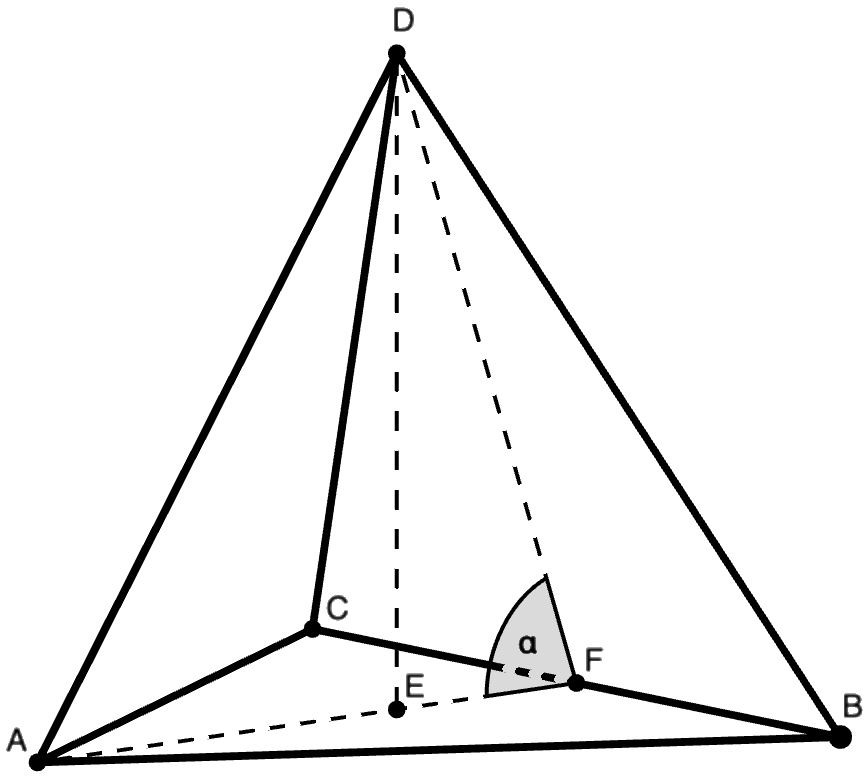
\includegraphics[scale=0.2]{RegulTetraeder}
		\caption{Ein regulärer Tetraeder}
		\label{Abb.4}
	\end{figure}
	
	\begin{proposition} \label{prop:irr}
		Für alle ungeraden $n\in\setN$ mit $n\geq 3$ gilt, $\frac{1}{\pi}\arccos\left(\frac{1}{\sqrt{n}}\right)$ ist irrational.
	\end{proposition}
	
	\begin{proof}
		Zuerst stellen wir fest, dass mit dem Additionstheorem
		\[\cos(\alpha)+\cos(\beta)=2\cos(\frac{\alpha+\beta}{2})\cos(\frac{\alpha-\beta}{2}) \]
		für $\alpha=(k+1)\varphi$ und $\beta=(k-1)\varphi$ gilt
		\begin{align*}
			\cos\left((k+1)\varphi\right)+\cos\left((k-1)\varphi\right)=&2\cos\left(\frac{(k+1)\varphi+(k-1)\varphi}{2}\right)
			\cos\left(\frac{(k+1)\varphi-(k-1)\varphi}{2}\right) \\
			=& 2\cos(k\varphi)\cos(\varphi)
		\end{align*}
		und damit folgt
		\begin{align}
			\cos((k+1)\varphi)=2\cos(k\varphi)\cos(\varphi)-\cos((k-1)\varphi). \label{prop:irr;1}
		\end{align}
		Wir definieren uns nun $\varphi_n=\arccos(\frac{1}{\sqrt{n}})$ für $n=2m+1$ mit $m\in\setN$. Dann ist 
		$\cos(\varphi_n)=\frac{1}{\sqrt{n}}$ und $0\leq\varphi_n\leq\pi$. \\
		Mit Induktion über $k\in\setN_0$ zeigen wir, dass gilt
		\begin{align}
			\cos(k\varphi_n)=\frac{A_k}{\sqrt{n}^k}, \label{prop:irr;2}
		\end{align}
		wobei $A_k$ eine ganze Zahl ist, die nicht durch $n$ teilbar ist. Wir beginnen und stellen fest, dass
		\begin{align*}
			&\text{für $k=0$}\qquad 1=\cos(0\cdot\varphi_n)=\frac{A_0}{\sqrt{n}^0}=A_0 \\
			&\text{für $k=1$}\qquad \frac{1}{\sqrt{n}}=\cos({1\cdot\varphi_n})=\frac{A_1}{\sqrt{n}^1}=\frac{A_0}{\sqrt{n}}
		\end{align*}
		und damit $A_0=A_1=1$ ist. Weiterhin gilt mit \ref{prop:irr;1}
		\begin{align*}
			\cos((k+1)\varphi_n)=& 2\cos(k\varphi_n)\cos(\varphi_n) -\cos((k-1)\varphi_n) \\
			=&2\frac{A_k}{\sqrt{n}^k}\cdot\frac{1}{\sqrt{n}}-\frac{A_{k-1}}{\sqrt{n}^{k-1}} \\
			=&\frac{\overbrace{2 A_k-nA_{k-1}}^{=:A_{k+1}}}{\sqrt{n}^{k+1}}.
		\end{align*}
		Da $A_k$ nicht durch $n$ teilbar ist und $n\geq 3$ ungerade, ist die Zahl $2A_k$ auch nicht durch $n$ teilbar 
		und damit auch nicht $A_{k+1}:=2 A_k -nA_{k-1}$. Wir haben also eine konkrete Darstellung für $A_{k+1}$ 
		gefunden und sind mit der Induktion fertig. \\
		Nun kommen wir zum eigentlichen Beweis. Angenommen $\frac{1}{\pi}\varphi_n$ ist 
		rational mit
		\[\frac{1}{\pi}\varphi_n=\frac{m}{k}\]
		für $m\in\setZ$ und $k\in\setN$. Dann gilt mit $k\varphi_n=m\pi$ und \ref{prop:irr;2}
		\[\pm 1=\cos(m\pi)=\cos(k\varphi_n)=\frac{A_k}{\sqrt{n}^k}. \]
		Also auch $\sqrt{n}^k=\pm A_k$ und da $A_k$ eine ganze Zahl ist, ist $\sqrt{n}^k$ auch eine und somit 
		$k\geq 2$. Damit ist jedoch $n$ ein Teiler von $\sqrt{n}^k$ und da $\sqrt{n}^k \vert A_k$, teilt $n$ auch 
		$A_k$, was ein Widerspruch ist.
	\end{proof}
	
	Damit folgt also für $n=9$, dass $\arccos\left(\frac{1}{3}\right)$ nicht in $\pi\setQ$ liegt. Wir erhalten unser 
	folgendes Resultat.
	
	\begin{corollary}[Dehns Lösung]
		Sei $Q$ ein Quader und $T$ ein regulärer Tetraeder mit gleichem Volumen und Kantenlänge $l$. 
		Dann gilt nach Beispiel \ref{exp:quader} $D(Q)=0$ und nach Beispiel \ref{exp:regTetr}
		\[D(T)=6l\otimes_{\setZ}\arccos\left(\frac{1}{3}\right).\]
		Da nach Proposition \ref{prop:irr} $\frac{1}{\pi}\arccos\left(\frac{1}{3}\right)$ irrational ist, liegt
		$\arccos\left(\frac{1}{3}\right)$ nicht in $\pi\setQ$ und damit ist nach Bemerkung \ref{bem:dehn=0} 
		mit $l\neq 0$ auch $6l\otimes_{\setZ}\arccos\left(\frac{1}{3}\right)\neq 0$. Also gilt
		\[ D(Q)=0\neq 6l\otimes_{\setZ}\arccos\left(\frac{1}{3}\right)=D(T).\]
		Also sind $Q$ und $T$ nicht zerlegungsgleich.
		% und
		%
		%...
		%
		% damit auch nicht ergänzungsgleich.
	\end{corollary}
	
	%
	%Wir werden im folgenden immer kommutative Ringe mit Eins betrachen.
	%
	%\begin{remark}
	%	Sei $R$ ein kommutativer Ring mit Eins und seien $M$ und $N$ zwei $R$-Moduln. Dann betrachten wir 
	%	zunächst die Elemente $(m,n)$ der Menge $M\times N$. Diese Menge erzeugt einen freien Modul 
	%	$R^{(M\times N)}$, dessen Elemente typischerweise eine Linearkombination der Form
	%	\[ \sum_{i=1}^n (m_i,n_i)\cdot r_i \]
	%	sind, wobei für alle $i=1,\ldots,n$ gilt $m_i\in M$, $n_i\in N$ und $r_i\in R$.
	%	Wir möchten nun für Elemente $m,m'\in M$, $n,n'\in N$ und $r,r'\in R$ gerne identifizieren:
	%	\begin{align*}
	%		(mr+m'r',n)\quad \text{mit}&\quad (m,n)\cdot r +(m',n)\cdot r' \\
	%		\text{und } (m,nr+n'r') \quad \text{mit}&\quad (m,n)\cdot r+(m,n')\cdot r'.
	%	\end{align*}
	%	Die Idee hierfür ist, dass für eine bilineare Abbildung $f$ beispielsweise gilt $f(m+m',n)=f(m,n)+f(m',n)$. 
	%	Um dies so durchzuführen, dass wir am Ende wieder ein Modul erhalten, betrachten wir in $R^{(M\times N)}$ 
	%	Elemente der Form
	%	Nun teilen wir den von ihnen erzeugten Untermodul heraus und erhalten einen Modul, der von den 
	%	Paaren $(m,n)\in M\times N$ erzeugt wird und in dem die obigen Relationen gelten.
	%\end{remark}
	%
	%\begin{definition}[Tensorprodukt]
	%	Sei $R$ ein kommutativer Ring mit Eins und seien $M$, $N$ zwei $R$-Moduln. Dann definieren wir 
	%	das \textsl{Tensorprodukt} von $M$ und $N$ über $R$ durch
	%	\[ M\times_R N= R^{(M\times N)}/\langle T \rangle, \]
	%	wobei die Menge $T\subset R^{(M\times N)}$ von Relationen definiert ist 
	%	\begin{align*}
	%		T =& \{ (m+m',n)-(m,n)-(m',n)\ \vert\ m,m'\in M, n\in N\} \\
	%		\cup& \{ (mr,n)-(m,n)\cot r \ \vert\ m\in M, n\in N, r\in R\} \\
	%		\cup& \{ (
	%
	%\section{Zerlegungsgleichheit von Polyedern; Bricard}
	%
	%
	%
	%\section{Ausblicke}
	%
	%Im folgenden wollen wir uns anschauen, ob es ähnliche Resultate auch im sphärischen oder hyperbolischen Raum 
	%gibt.
	%
	%\subsection{Zerlegungsgleichheit im Sphärischen}
	%
	%\subsection{Zerlegungsgleichheit im Hyperbolischen}
	%
\end{document}